%!TEX root = ../proteoform_suite_manual.tex
%---------------------------------------------------------------------
%	EXPERIMENT Theoretical	EXPERIMENT COMPARISON
%---------------------------------------------------------------------

\section{Experiment Experiment Comparison}

\subsection{Overview}

On this page, experimental proteoforms are compared to one another, generating a list of experiment-experiment pairs. Each experiment-experiment pair has a mass difference between the two experimental proteoforms in the pair. A histogram is generated of the mass differences for all experiment-experiment pairs; experiment-experiment pairs in accepted delta mass peaks are used to construct proteoform families. Experiment-false pairs are generated from experimental proteoforms with a different number of lysines (NeuCode labeled) or from proteoforms eluting at a different retention times (unlabeled); these pairs are used to estimate a false discovery rate for each delta mass peak. 

\subsection{Run Page}
\begin{itemize}
\item The Theoretical Proteoforms and Aggregated Proteoforms pages must be run before running this page.
\item Set all parameters as desired for current analysis (see below)
\item Click Run Page button (top right)
\item Browse the list of delta mass peaks from the histogram of experiment-experiment pairs delta masses (top left table). Accept peaks that have an acceptable false discovery rate and correspond to common/likely modifications. 
\end{itemize}

\subsection{Set Parameters}
\begin{figure}[h]
\centering
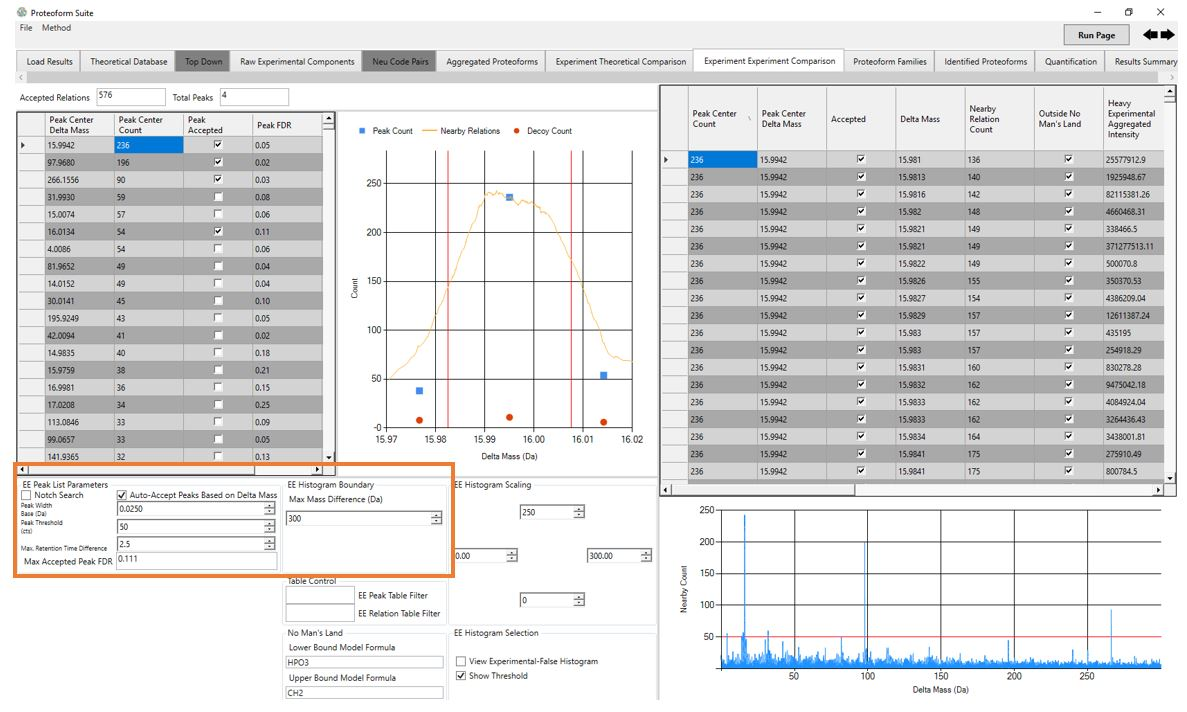
\includegraphics[scale=0.43]{figures/ee1.jpg}
\end{figure}
\begin{itemize}
\item Notch Search: if checked, a notch search will be performed. For each modification, experiment-experiment pairs will be generated if the delta mass is within the set tolerance from the modification's delta mass
\item Auto-Accept Peaks Based on Delta Mass: if checked, peaks with a count above the Peak Threshold will be accepted if they correspond to a common modification
\item Peak Width Base (Da): if notch search is unchecked, this is the size of bins used for generating the delta mass histogram from experiment-experiment pair delta masses
\item Peak Threshold (cts): the minimum number of experiment-experiment pairs that must belong to a delta mass peak for the peak to be accepted
\item Max. Retention Time Difference: maximum allowed retention time difference for two experimental proteoforms to be eligible to be in an experiment-experiment pair
\item Notch Tolerance: if a notch search is performed, this tolerance will be used to generate experiment-experiment pairs at each modification delta mass
\item EE Histogram Boundary: maximum delta masses to be considered for an experiment-experiment pair to be generated 
\end{itemize}

\subsection{Results}
\begin{itemize}
	\item Accepted Relations: the number of accepted experiment-experiment pairs
	\item Total Peaks: the number of accepted experiment-experiment delta mass peaks
	\item Experiment-Experiment Delta Mass Peaks table: the top left table displays the delta mass peaks from the histogram of experiment-experiment pair delta masses. If a notch search is performed, each peak is a different modification delta mass/notch
	\begin{figure}[h]
\centering
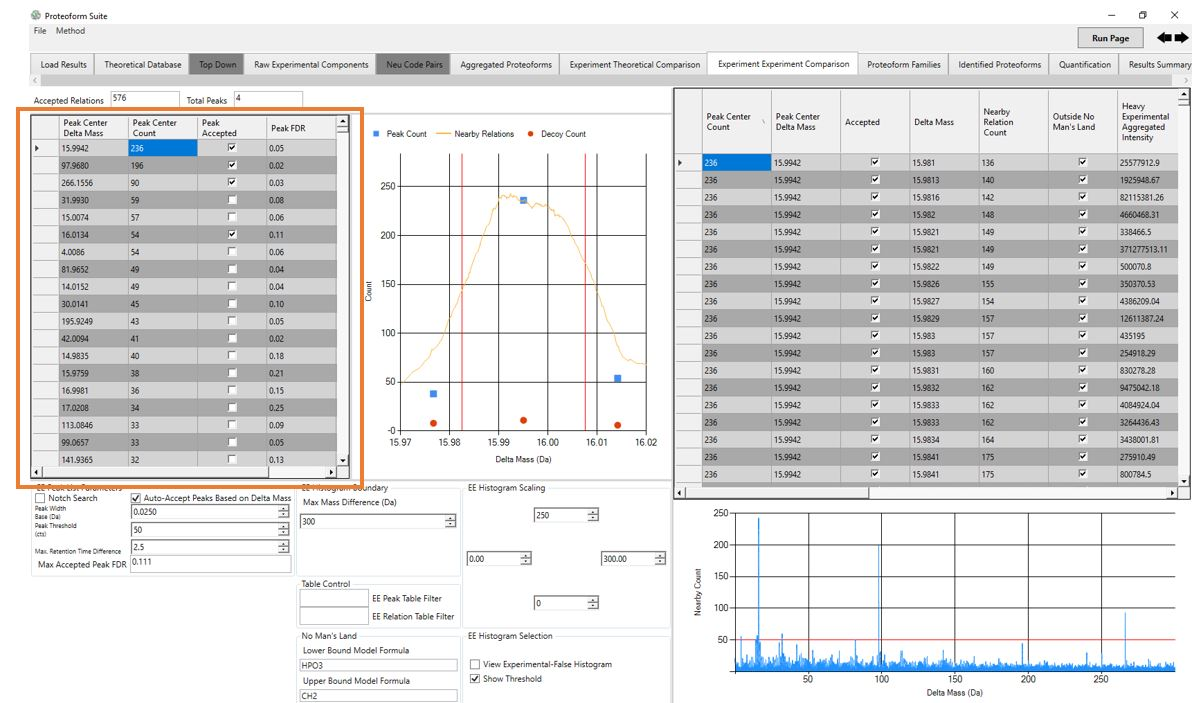
\includegraphics[scale=0.43]{figures/ee2.jpg}
\end{figure}
	\begin{itemize}
		\item Peak Center Delta Mass: delta mass at the center of this delta mass peak 
		\item Peak Center Count: the number of experiment-experiment comparisons delta masses that are part of this peak
		\item Peak Accepted: checked if peak is accepted (peak center count is above peak threshold in set parameters or manually changed by user). This check box can be checked or unchecked to accept or unaccept a delta mass peak
		\item Peak FDR: the false discovery rate for this delta mass peak; determined based on the number of experiment-false pairs that fall within this peak delta mass plus/minus half of the peak width base
		\item Peak Assignment Possibilities: modifications/combinations of modifications that could correspond to the delta mass of this delta mass peak
		\end{itemize}
	\item Experiment-Experiment Delta Mass Peak Zoom-in Graph: when a peak is selected in the Experiment-Experiment Delta Mass Peak table, this top left graph displays a zoom-in of the peak from the Experiment-Experiment Delta Mass Histogram (bottom right graph). Blue square point is peak count, and yellow circle point is median decoy count for this peak. The red line plots the nearby relations histogram count for each delta mass value
		\begin{figure}[h]
\centering
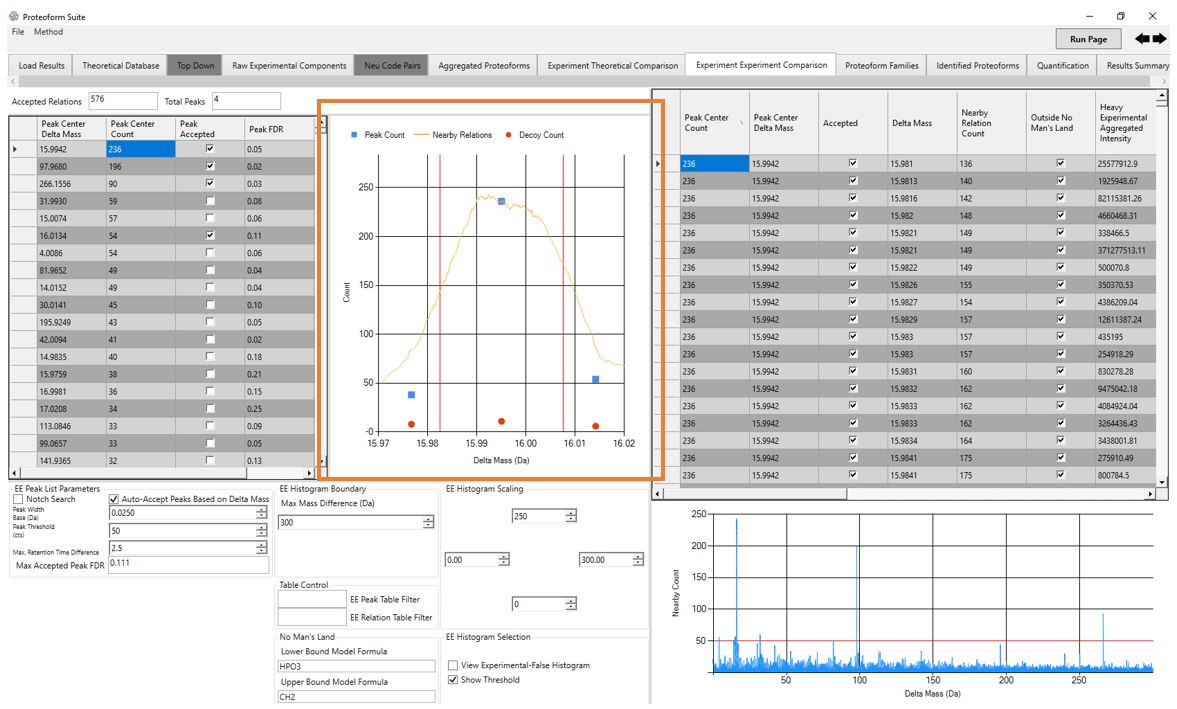
\includegraphics[scale=0.44]{figures/ee3.jpg}
\end{figure}
\pagebreak
\item {Experiment-Experiment Pairs}: this right table displays all experiment-experiment pairs, consisting of two experimental proteoforms and their mass difference.
		\begin{figure}[h]
\centering
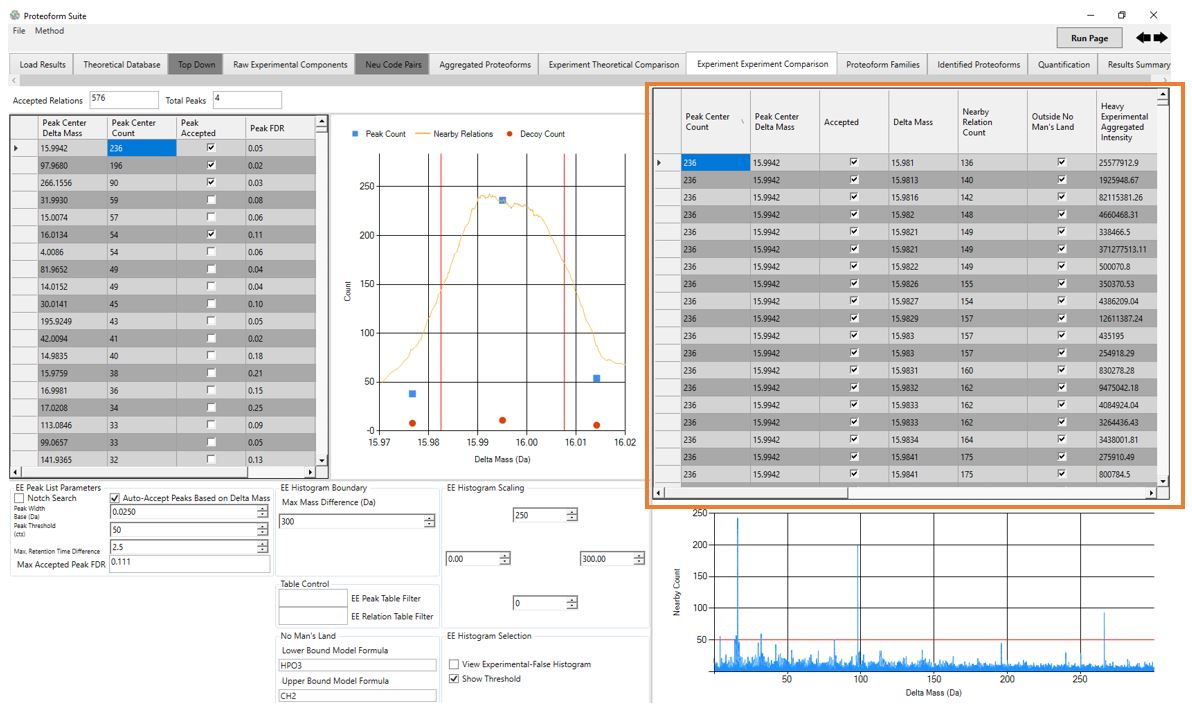
\includegraphics[scale=0.44]{figures/ee4.jpg}
\end{figure}
\begin{itemize}
	\item Peak Center Count: if this pair is in a delta mass peak, the number of pairs in the peak
	\item Peak Center Delta Mass: if this pair is in a delta mass peak, the delta mass at the center of the peak
	\item Accepted: checked if this pair is in a delta mass peak that is accepted in the Experiment-Experiment Delta Mass Peaks table
	\item Delta Mass: mass difference between the two experimental proteoforms in this pair
	\item Nearby Relation Count: number of pairs with a delta mass close to this pair's delta mass; this value is used to plot the delta mass histogram
	\item Outside No Man's Land: checked if this pair is an acceptable delta mass regarding the numbers after the decimal point. Pairs with a delta mass in no man's land are not joined into delta mass peaks
	\item Heavy Experimental Aggregated Intensity: sum of intensity of aggregated raw experimental components for the heavier experimental proteoform in this pair
	\item Aggregated RT Heavy: retention time of heavier experimental proteoform in this pair
	\item Number Heavy Experimental Observations: number of aggregated raw experimental components (unlabeled) or NeuCode pairs (NeuCode labeled) for the heavier experimental proteoform in this pair. If top-down proteoform, the number of top-down hits
	\item Heavy Experimental Aggregated Proteoform Mass: mass of the heavier experimental proteoform in this pair
	\item Heavy Experimental Accession: unique ID given by Proteoform Suite for the heavier experimental proteoform in this pair		
	\item Heavy Abundant Exp. Component for Manual Validation: file information for the most abundant raw experimental component aggregated into the heavier experimental proteoform of this pair
	\item Light Experimental Aggregated Intensity: sum of intensity of aggregated raw experimental components for the lighter experimental proteoform in this pair
	\item Aggregated RT Light: retention time of lighter experimental proteoform in this pair
	\item Number Light Experimental Observations: number of aggregated raw experimental components (unlabeled) or NeuCode pairs (NeuCode labeled) for the lighter experimental proteoform in this pair. If top-down proteoform, the number of top-down hits
	\item Light Experimental Aggregated Proteoform Mass: mass of the lighter experimental proteoform in this pair
	\item Light Experimental Accession: unique ID given by Proteoform Suite for the lighter experimental proteoform in this pair		
	\item Light Abundant Exp. Component for Manual Validation: file information for the most abundant raw experimental component aggregated into the lighter experimental proteoform of this pair
\end{itemize}
\item Experiment-Experiment Delta Mass Histogram graph: this bottom right graph shows a histogram of the delta masses for the experiment-experiment pairs
\begin{figure}[h]
\centering
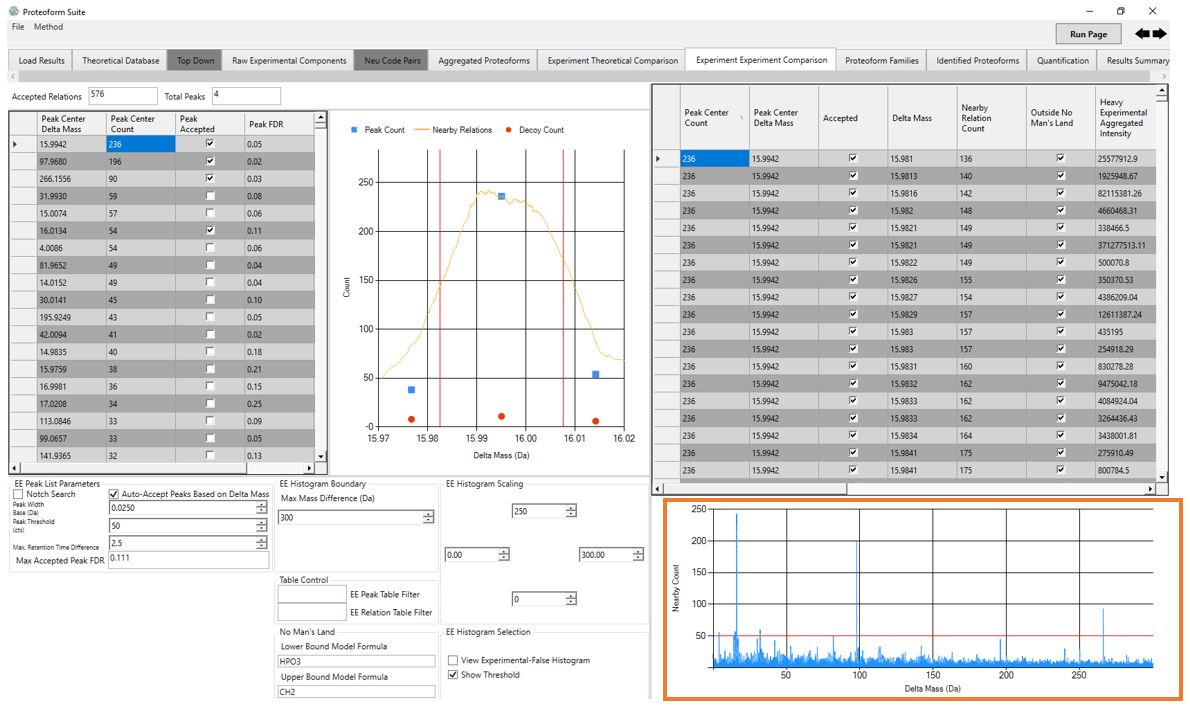
\includegraphics[scale=0.46]{figures/ee5.jpg}
\end{figure}
\begin{itemize} 
	\item View Experiment-False Histogram: if checked, delta mass histogram for experiment false pairs will be plotted
	\item Show Threshold: if checked, a red line on the graph shows the Peak Threshold set
	\end{itemize}
\end{itemize}